% This template was initially provided by Dulip Withanage.
% Modifications for the database systems research group
% were made by Conny Junghans,  Jannik Strötgen and Michael Gertz

\documentclass[
     12pt,         % font size
     a4paper,      % paper format
     BCOR10mm,     % binding correction
     DIV14,        % stripe size for margin calculation
     ]{article}

%%%%%%%%%%%%%%%%%%%%%%%%%%%%%%%%%%%%%%%%%%%%%%%%%%%%%%%%%%%%

% PACKAGES:

% Use German
\usepackage[english]{babel}
% Input and font encoding
\usepackage[utf8]{inputenc}
\usepackage[T1]{fontenc}
% Index-generation
\usepackage{makeidx}
% Embedding of URLs
\usepackage{url}
% Special \LaTex symbols (e.g. \BibTeX)
%\usepackage{doc}
% Include Graphic-files
\usepackage{graphicx}
% Include doc++ generated tex-files
%\usepackage{docxx}
% Fuer anderthalbzeiligen Textsatz
\usepackage{setspace}
\usepackage[table,xcdraw]{xcolor}
\usepackage{hhline}
\usepackage{highlight}

\usepackage{biblatex}
\bibliography{references.bib}

% hyperrefs in the documents
\PassOptionsToPackage{hyphens}{url}\usepackage[bookmarks=true,colorlinks,pdfpagelabels,pdfstartview = FitH,bookmarksopen = true,bookmarksnumbered = true,linkcolor = black,plainpages = false,hypertexnames = false,citecolor = black,urlcolor=black]{hyperref}
%\usepackage{hyperref}


% CUSTOM:

% For Quotes:
\usepackage{csquotes}

% For Definitions:                   						
\usepackage{amsthm}
\usepackage[framemethod=tikz]{mdframed}

\newtheoremstyle{defi}
{\topsep}         % Abstand oben
{\topsep}         % Abstand unten
{\normalfont}     % Schrift des Bodys
{0pt}             % Einschub der ersten Zeile
{\bfseries}       % Darstellung von der Schrift in der �berschrift
{:}               % Trennzeichen zwischen �berschrift und Body
{.5em}            % Abstand nach dem Trennzeichen zum Body Text
{\thmname{#3}}    % Name in eckigen Klammern
\theoremstyle{defi}

\newmdtheoremenv[
hidealllines = true,       % Rahmen komplett ausblenden
leftline = true,           % Linie links einschalten
innertopmargin = 0pt,      % Abstand oben
innerbottommargin = 4pt,   % Abstand unten
innerrightmargin = 0pt,    % Abstand rechts
linewidth = 3pt,           % Linienbreite
linecolor = gray!40,       % Linienfarbe
]{defStrich}{Definition}     % Name der des formats "defStrich"

% For Abbreviations:
\usepackage{acronym}

%For Mathematical LaTeX Macros
\usepackage{mathtools}
\DeclarePairedDelimiter\abs{\lvert}{\rvert}%
\DeclarePairedDelimiter\norm{\lVert}{\rVert}%

% For subfigures
\usepackage{caption}
\usepackage{subcaption}

%%%%%%%%%%%%%%%%%%%%%%%%%%%%%%%%%%%%%%%%%%%%%%%%%%%%%%%%%%%%

% OTHER SETTINGS:

% Choose language
\newcommand{\setlang}[1]{\selectlanguage{#1}\nonfrenchspacing}


\begin{document}

% TITLE:
\pagenumbering{roman} 
\begin{titlepage}

\vspace*{1cm}
\begin{center}
\textbf{ 
\Large Heidelberg University\\
\smallskip
\Large Institute of Computer Science\\
\smallskip
}

\vspace{3cm}

\textbf{\large Project proposal for the lecture Advanced Machine Learning}

\vspace{0.5\baselineskip}
{\huge
\textbf{Project ideas in the area of Covid-19 research}
}
\vspace{0.5cm}

\url{https://github.com/nilskre/AML-covid-project}

\end{center}

\vfill 

{\large
\begin{tabular}[l]{ll}
Team Member: & Felix Hausberger, 3661293,\\
  & Applied Computer Science\\
  & eb260@stud.uni-heidelberg.de\\
  & \\
Team Member: & Nils Krehl, 3664130,\\
  & Applied Computer Science\\
  & pu268@stud.uni-heidelberg.de\\
  
\end{tabular}
}

\end{titlepage}

% \section*{Abstract}


%\section*{Plagiarism statement}

We certify that this report is our own work, based on our personal study and/or research and that we have acknowledged all material and sources used in its preparation, whether they be books, articles, reports, lecture notes, and any other kind of document, electronic or personal communication.

We also certify that this report has not previously been submitted for assessment in any other unit, except where specific permission has been granted from all unit coordinators involved, or at any other time in this unit, and that we have not copied in part or whole or otherwise plagiarized the work of other students and/or persons.

\newpage

%\section*{Member contributions}

\subsubsection*{Nils Krehl}

Came up with the project idea and was the domain expert for the project's biomedical domain. Initial research for the topic and feasibility analysis.
Extensive research in the areas of the project's overall composition, related work on mutation prediction, molecular biological basics, data sources, dataset creation and dataset insights.
Responsible for the data selection and download, the dataset creation, the generation of dataset insights and the pretraining and evaluation of the Transformer model.


\subsubsection*{Felix Hausberger}

Extensive research in the area of machine learning models, especially the connection between \ac{NLP} methods and our project, previous work on mutation prediction and different model ar\-chi\-tec\-tu\-res such as \ac{Seq2Seq}, Transformer and \acp{GAN}.
Responsible for the data preprocessing, the model ar\-chi\-tec\-tu\-re, implementation and configuration, the GAN training and evaluation.

\newpage
\tableofcontents
\newpage

\pagenumbering{arabic}

\section*{List of Abbreviations}

\begin{acronym}[WYSISWG]

	\acro{GAN}{Generative Adversarial Network}
	\acro{LSTM}{Long Short-Term Memory}
	\acro{RNN}{Recurrent Neural Network}

\end{acronym}
%\section{Introduction}  \label{introduction}

% Motivation: See MutaGAN paper

% Our novelties: 
% - Bigger dataset compared to previous papers
% - New architecture based on transformers and a GAN framework

\newpage

\section{Machine Learning based prediction of the next SARS-CoV-2 variants and simulation of vaccine effectiveness} \label{proposal1}

\textbf{1. Idea and research question}

There is hope for an end of the pandemic due to the vaccines. All vaccines are developed against the wild type of the virus. Through the mutation processes the danger, that a variant occurs, against which the vaccines  are no longer effective, arises (viral escape). This proposal aims to detect this development faster to enable a faster and better response to new variants. So there are two scientific questions (which can also be separated):

\begin{enumerate}
	\item Can the next possible SARS-CoV-2 variants be predicted by a \ac{ML} model?
	\item Based on the  predicted possible next variants can the effectiveness of the vaccines be simulated?
\end{enumerate}

\color{green}
It is more realistic to focus on one of the questions above. For the first the data access is easier.
\color{black}

\textbf{2. Related work}

Already some works exist in the area of predicting virus mutations using \ac{ML} techniques. Hie et al. \cite{Hie2021} applied methods developed for \ac{NLP}.  According to their work escape mutations look different to the immune system, but have the same viral infectivity. The analogy from the \ac{NLP} area are word changes, which change the meaning of a sentence, but the grammaticality remains. %Through their work, they have managed to generate a connection between natural language and viral evolution. 
Even before the SARS-CoV-2 pandemic, research was done in this area, e.g. from Salama et al. \cite{Salama2016}. They used neural networks for predicting new mutations and rough set techniques for detecting patterns in mutations. Furthermore they validated their approach for the Newcastle virus and achieved an accuracy of 75\%. \ac{GAN} achieve great results in image generation. Berman et al. applied a \ac{GAN} in \cite{Berman2020} to generate \ac{DNA} sequences.

\textbf{3. Approach}

After preprocessing the raw SARS-CoV-2 genomes we would like to train a \ac{ML} model for predicting the probable next mutations. The \ac{ML} model could be a standard neural network (as in  \cite{Salama2016}), a GAN (as in \cite{Berman2020}) or a neural network language model (as in \cite{Hie2021}). Due to a lack of time we haven't decided yet for one \ac{ML} model.
\color{green}
Is clarified after a decision for one proposal.
\color{black}

\textbf{4. Data sources}

For predicting the next possible SARS-CoV-2 variants the SARS-CoV-2 genome develop\-ment from the past can be used as data source (genomic time series data). Data sources are available through the GISAID initiative \cite{Gisaid2021}. In April 2021 over one million SARS-CoV-2 genomes are available via GISAID \cite{Maxmen2021}. Based on this data the Nextstrain\footnote{https://nextstrain.org/ncov/global?label=clade:19A} project provides a visualization how the SARS-CoV-2 genome evolves.

%In terms of data quality, when working with genomic data one should always have in mind, that genotyping errors are possible.

\textbf{5. Computational resources}

The needed computational resources and time depends on the concrete chosen \ac{ML} approach. As described above due to a lack of time we haven't decided yet for one \ac{ML} approach. For further research and the decision for one \ac{ML} approach we keep this in mind.

\textbf{6. Probable difficulties}

Challenges could arise due to the amount of data (one SARS-CoV-2 genome consists of about 30.000 bases => TS size = data instances * 30.000). This can be encountered with less data instances or a compression of SARS-CoV-2 genome e.g. through DNA2vec \cite{Ng2017} (represents pieces of \ac{DNA} as vector).

\newpage

% ...
%\section{Conclusion} \label{conclusion}

Coming to a conclusion, our main research question was whether a \ac{ML} model can be trained to predict the next possible \ac{SARS-CoV-2} mutations.
The short answer to this is, that our trained \ac{ML} model is definitely able to generate possible next sequences. The pretraining of the transformer achieved a BLEU score of 0.8559 and the training of the \ac{GAN} achieved a BLEU score of TODO.

Based on related works introduced in chapter \ref{fundamentals}, we decided for a \ac{ML} model architecture consisting of a transfomer based \ac{GAN} Framework. This architecture was influenced by Berman et al. \cite{Berman2020}. Our novelity is the usage of transformers instead of \ac{LSTM}. This enables faster training, because transformers can be trained in parallel. 

For answering our research question we created a new dataset based on raw data from \ac{GISAID}. As part of this we developed a reusable pipeline for creating evolutionary datasets.

Another novelty is the application and training of such an \ac{ML} architecture for \ac{SARS-CoV-2}.

%TODO: Wie schneiden wir im vergleich zu den anderen arbeiten ab?
%TODO: is it really that convincing?

\vspace{0.5cm}

As an outlook, there are some improvements and further investigations we would like to evaluate in future work. As realized while generating data insights of the dataset, lots of our data instances are very similar to each other. To really model the worldwide development of \ac{SARS-CoV-2} mutation events, the raw dataset should be based on a subsampling of all available global data instances. Further improvements could be achieved by using a computing cluster for generating a larger dataset and for training the model on the full \ac{SARS-CoV-2} genome and not on a subset of the genome. Moreover in the model evaluation more domain specific metrics as proposed by Berman et al. \cite{Berman2020} could be used in addition to the BLEU score.


%\setcounter{section}{-1}
\section{Project Setup} \label{setup}
% TODO: Update

For a detailed description of how to set up the project, please have a look at \url{https://github.com/nilskre/bomberman_rl/blob/master/README.md}.
%\section{Fundamentals and Related Work} \label{fundamentals}

\subsection{From Probabilistic Language Models to modeling Evolution Theory} \label{fundamentalsA}

A probabilistic language model tries to approximate the probability distribution 

\begin{equation}
	P(w_1, ..., w_n) = \Pi_{t=1}^{n} P(w_t | w_1, ..., w_{t-1})
\end{equation}

with $w_t$ being a word at position (time step) $t$ in a sentence of length $n$. To build language models \acp{RNN} were used to model such probability distributions. 

\begin{figure}[ht]
	\centering
	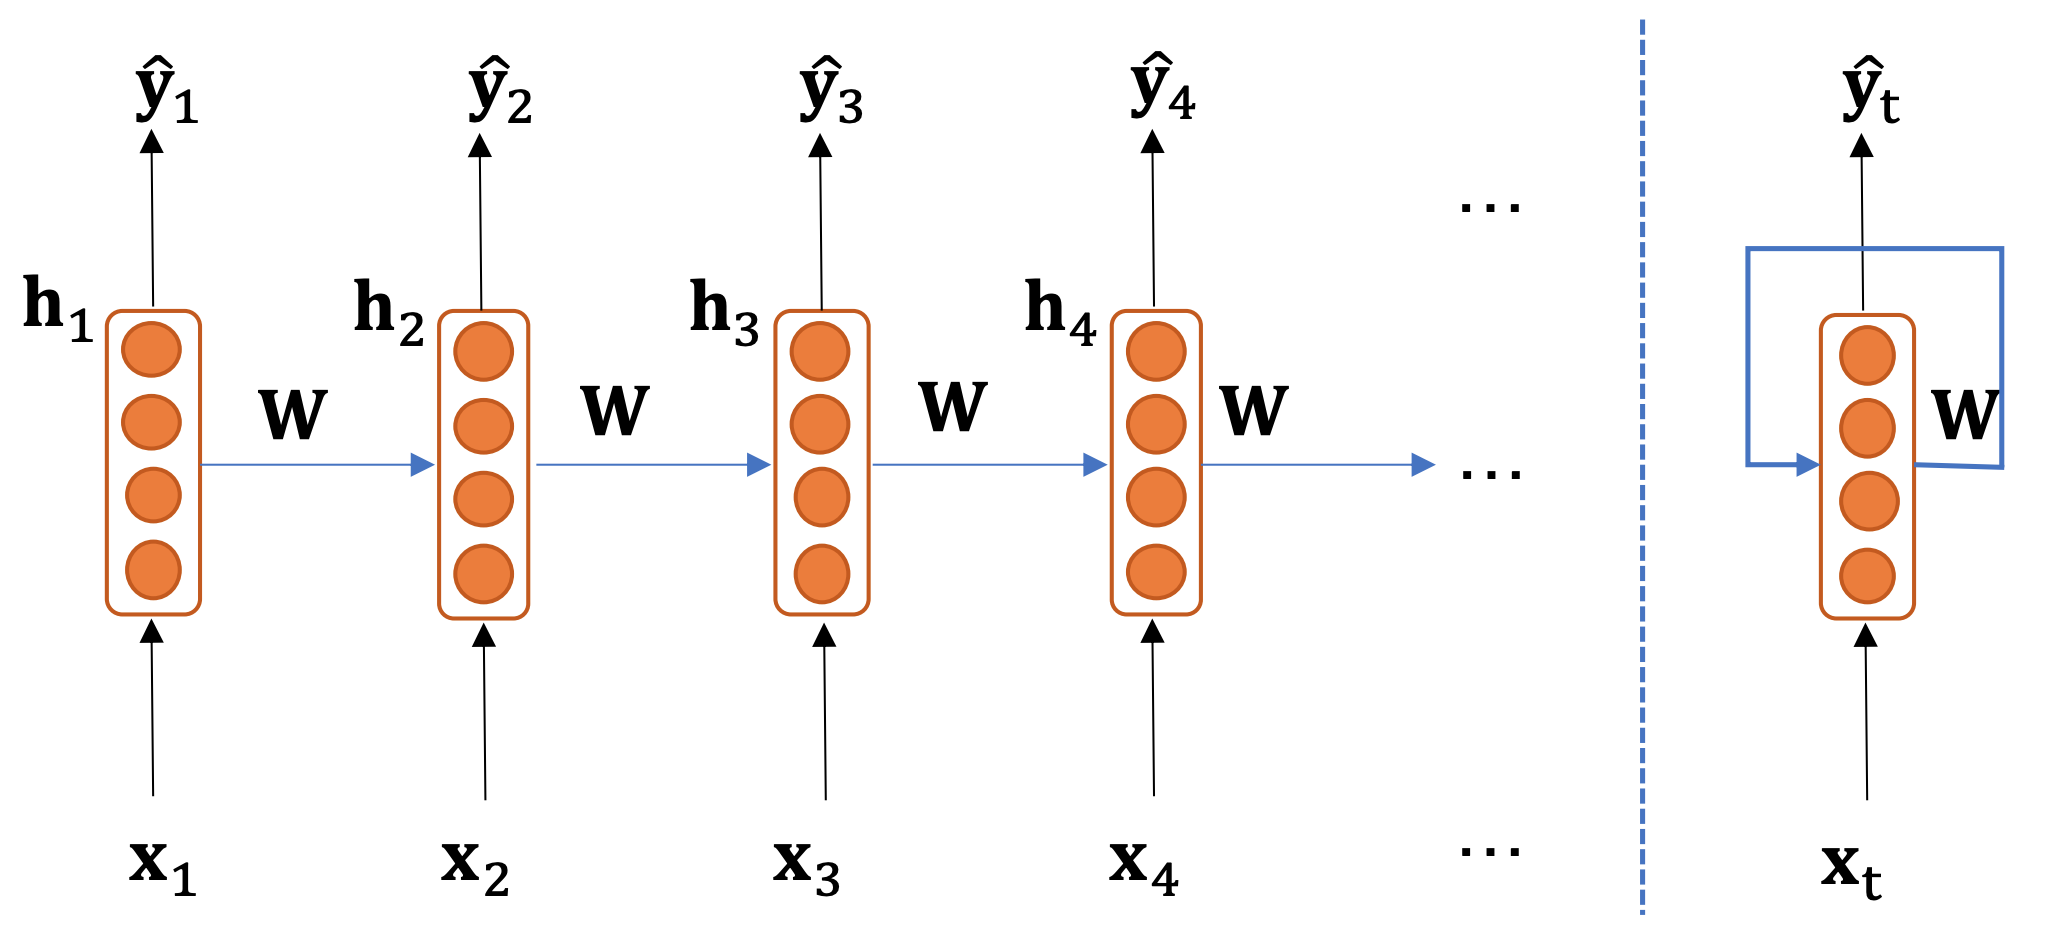
\includegraphics[width=0.8\linewidth]{figures/rnn_architecture.png}
	\caption{Architecture of a conventional \ac{RNN} \cite{Gertz2020}}
	\label{rnn_architecture}
\end{figure}

At each time step $t$ it outputs a probability distribution $P(w_t | w_1, ..., w_{t-1})$ given the words read so far in the current instance (see \autoref{rnn_architecture}). Words are read as a vectorized numerical representation, often given by pretrained so-called word embeddings $x_t$ which are lower dimensional and more semantically-enriched compared to simple one-hot encodings. One then calculates the hidden state $h_t$ by

\begin{equation}
	h_t = f(W^{(h)} h_{t-1} + W^{(x)} x_t + b_1)
\end{equation}

and the corresponding output porbability distribution by 

\begin{equation}
	\hat{y}_t = softmax(U^{(h)} h_t + b_2).
\end{equation}

The applied weight matrix is always the same for each time step $t$ giving the \ac{RNN} its name. One can therefore simplify the unrolled \ac{RNN} architecture on the left side of \autoref{rnn_architecture} to the one on the right, where the hidden state is continuously passed as an input to the next time step. To achieve a better convergence behavior during training, one can also provide the expected hidden state of time step $t-1$ instead of using the predicted hidden state, which is called teacher forcing. \acp{RNN} are able to process input of arbitrary length and are by their recurrent character capable to use information from previous time steps. Unfortunately, they are vulerable to vanishing and exploding gradient problems. \ac{LSTM} is a special \ac{RNN} architecture that solves such vulnerabilities by owning a separate long-term cell state besides a short-term hidden state and is introduces in \autoref{fundamentalsE}. It is able to preserve information over many time steps. \cite{Gertz2020}

\begin{figure}[ht]
	\centering
	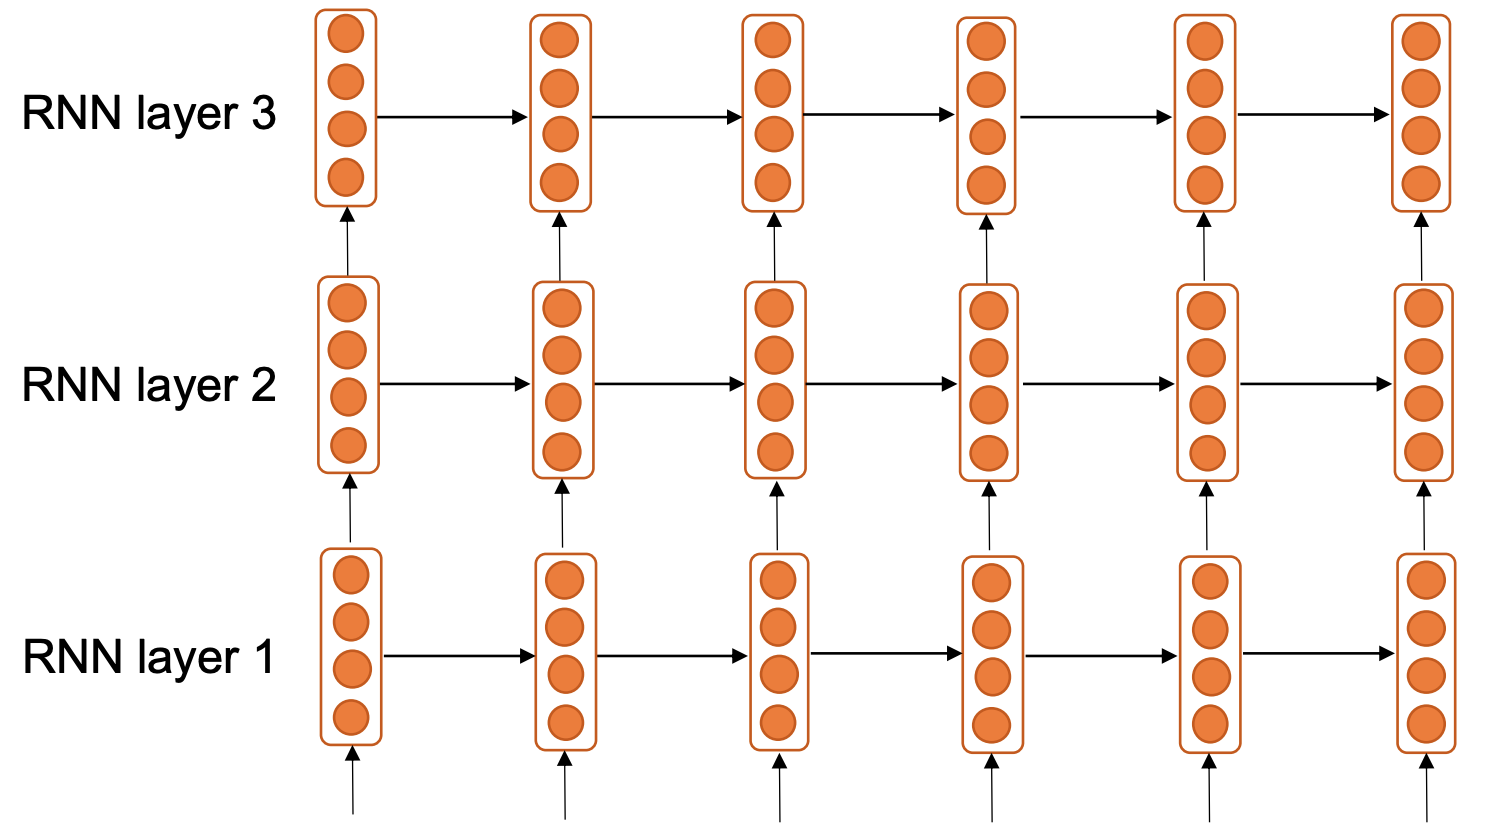
\includegraphics[width=0.8\linewidth]{figures/multi_layer_rnn.png}
	\caption{Architecture of a multi-layer  \ac{RNN} \cite{Gertz2020}}
	\label{multi_layer_rnn}
\end{figure}

One can also use two \acp{RNN}, one traversing a sentence from left to right and another one vice versa, with two different weight matrices to model the probability distribution bidirectionally. One therefore simply concatenates the hidden states of each \ac{RNN} before applying the the weight matrix $U$ and the $softmax()$ function. Also multi-layer \acs{RNN} can be utilized to generate higher-order features (hidden states) for the prediction task (see \autoref{multi_layer_rnn}). \cite{Gertz2020}

The \acp{RNN} or even better \acp{LSTM} architectures used for probabilistic language modeling can be reused in a more complex domain called sequence to sequence modeling for neural machine translation from one language to another. Here one first tries to learn a fixed-dimensional input representation from an input sequence using an encoder architecture based on an \ac{LSTM}. The so-called context vector is then decoded by a second \ac{LSTM} into a new sequence of words preserving the grammar but owning a different meaning. \cite{Sutskever2014}

Sequence to sequence models are introduced together with the \ac{LSTM} architecture in \autoref{fundamentalsE}. Here the connection to evolution theory can be drawn. \ac{RNA} sequences made of a concatenation of nucleotides \footnote{We restrict the representation of nucleotides solely to their nucleobases parts consisting of the distinct nucleobases guanine, adenine, cytosine and thymine. We therefore do not include the phosphate group and the five-carbon sugar components.} can be represented textually using the FASTA format. A sequence to sequence model can then transferably be applied in the domain of \ac{RNA} sequences to model how \ac{RNA}-based viruses change their structure to avoid the detection by the human immune system but still to preserve their infectivity and evolutionary fitness \cite{Hie2021}. 

\subsection{GISAID EpiFlu Data Platform} \label{fundamentalsB}

\subsection{Domain-Specific Methodologies to create Evolutionary  Datasets for Mutation Prediction} \label{fundamentalsC}

\subsection{Previous Work on Mutation Prediction} \label{fundamentalsD}

Even before the rise of Covid-19 there had been studies trying to predict mutations of \ac{RNA} viruses. In the collection of \cite{Wu2007, Yan2007, Wu2008} the authors predict the mutation positions in hemagglutinins from influenza A virus using logistic regression and plain neural networks and then use the resulting amino acid mutating probabilities to derive possible mutated amnio acids. The same approach is further used for H5N1 neuraminidase proteins. 

\cite{Salama2016} proved that nucleotides in an \ac{RNA} sequence can change based on their local neighborhood. Neural networks are used to predict new strains of the Newcastle virus and subsequently a rough set theory based algorithm is introduced to extract the according point mutation patterns. 

\cite{Mohamed2021} uses a more modern sequence to sequence approach based on \acp{LSTM} to learn nucleotide mutations between time-series species of H1N1 Influenza virus and the Newcastle virus as mutations can also be influenced by long-distance relations of amino acids. Therefore one hot-encoded \ac{RNA} sequences of a parent generation preprocessed to words is given as an input and the output is the predicted offspring generation evaluated by accuracy to the compared true offspring generation. The achieved accuracy in this paper is questionably high with 98.9\% on the H1N1 Influenza virus and 96.9\% on the Newcastle virus, possibly because of overfitting to the few 4.609 samples for H1N1 Influenza virus and only 83 for the Newcastle virus. Our approach therefore tries to increase the number of samples available for training when building the dataset. 

Our approach will neither use any of the just mentioned architectures, but uses a transformer based architecture coupled with a GAN-style training architecture. Nevertheless a short introduction into sequence to sequence models and the underlying long short-term memory components shall be given to better point out our architectural decisions . 

\subsection{Sequence to Sequence Models based on Long Short-Term Memory} \label{fundamentalsE}

% TODO: Figure Seq2Seq

The original \ac{LSTM} unit was introduced in \cite{Hochreiter1997} and can be used for language modeling instead of using plain \acp{RNN} to prevent running into vanishing or exploding gradient problems \cite{Sundermeyer2012}. The architecture of an \ac{LSTM} is shwon in the following figure:

\begin{figure}[ht]
	\centering
	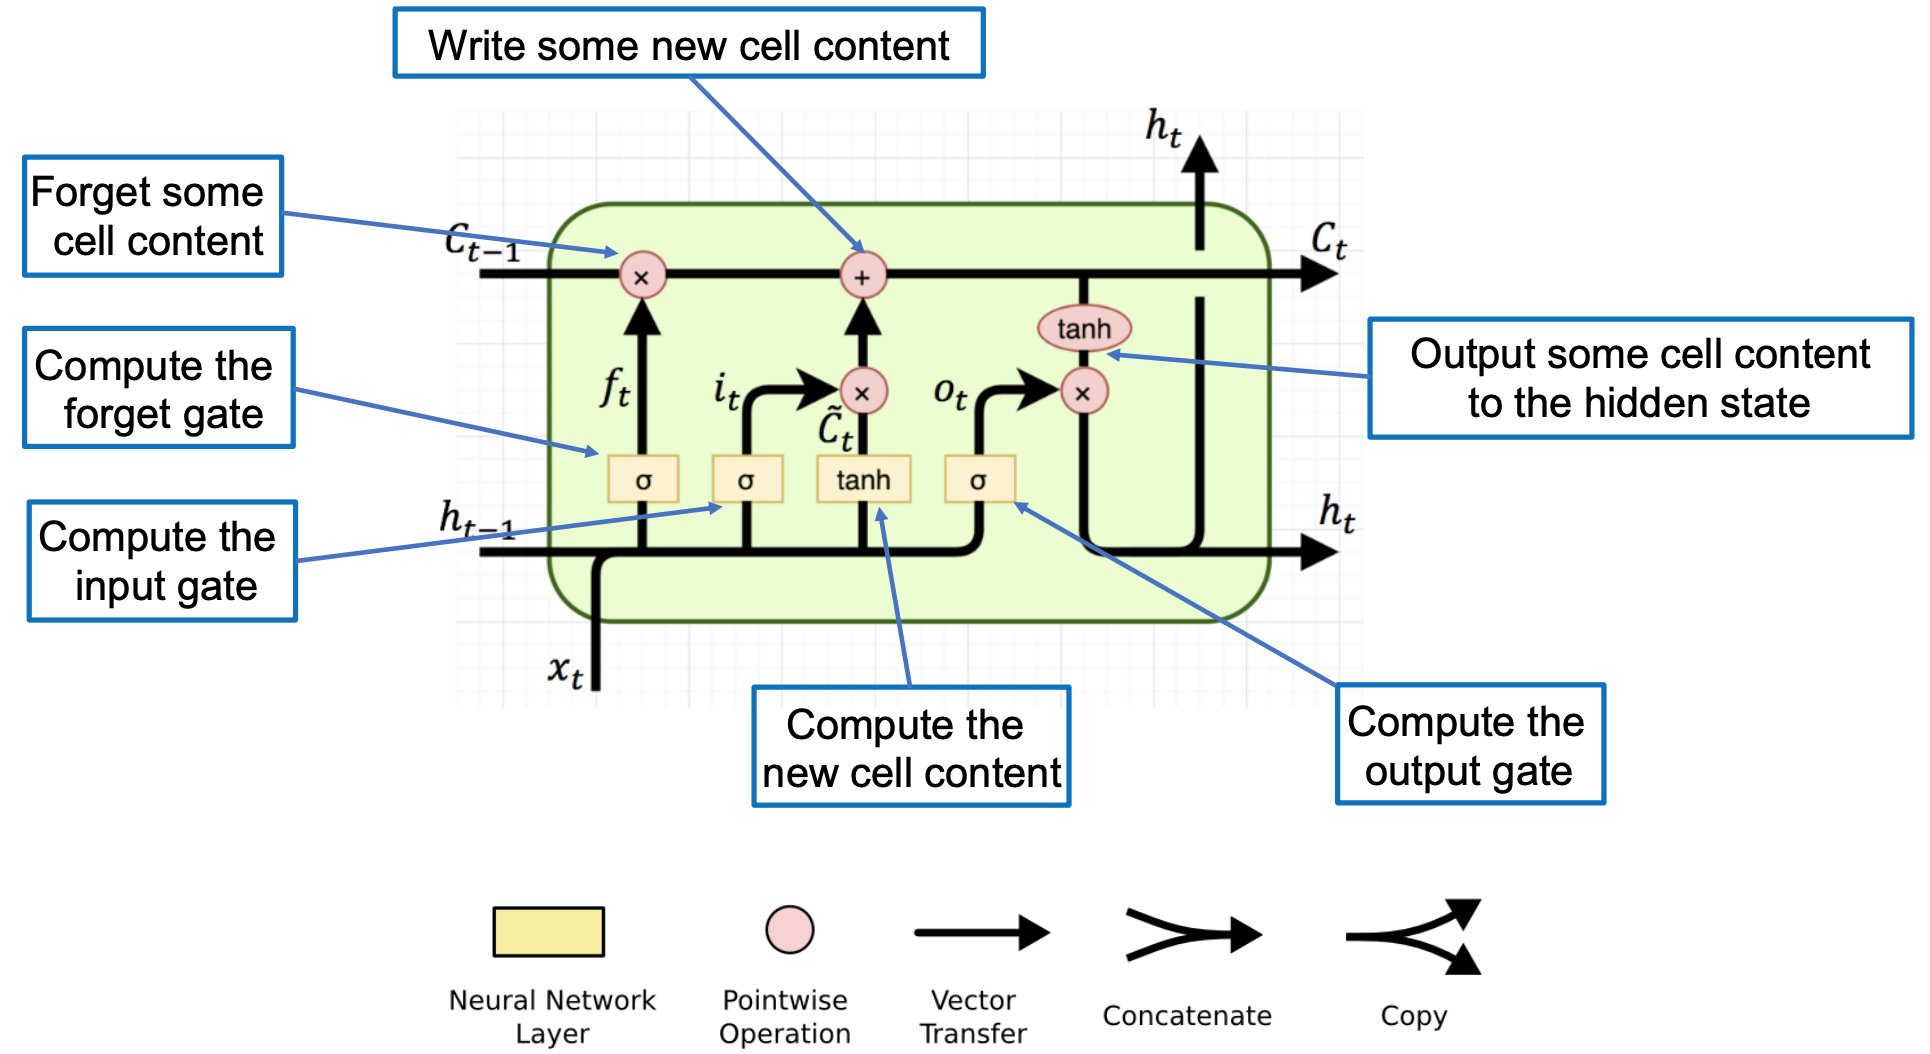
\includegraphics[width=\linewidth]{figures/lstm_architecture.png}
	\caption{Architecture of an \ac{LSTM} \cite{Gertz2020}}
	\label{lstm_architecture}
\end{figure}

It consists of a hidden state $h_t$ and an additional cell state $c_t$. The cell state stores long-term information and is used to derive a new hidden state. Information flows through three different gates inside the \ac{LSTM}. The forget gate is used to control which parts of the cell state are potentially carried on to the next time step, the input gate is responsible to decide which parts of the cell state should be updated and the output gate determines what is being passed on as the new hidden state. All three gates and depend on the previous hidden state and the current input. They provide factors limited to the interval [0,1] by the sigmoid function and are multiplied with the cell state, the changes to be added to the cell state and the new hidden state derived from the cell state. Through the cell state an \ac{LSTM} therefore makes it possible to capture long-distance dependencies. \cite{Gertz2020}

\cite{Sutskever2014} introduced sequence to sequence learning following a multi-layer encoder-decoder style model architecture. One layer consists of one \ac{LSTM} that is used as an encoder to learn a large fixed-dimensional vector representation of a size-unrestricted input sequence called the context vector. This vector consists of the last cell and hidden state of the encoder and incorporates the structure of the input sequence helping the followig decoder \ac{LSTM} to provide qualitative predictions for the output sequence. The second \ac{LSTM} therefore serves as a beam search\footnote{Do not choose the most probable word but the $B$ most likely word hypothesis and pass them to the next time step in the \ac{LSTM}. Whichever hypothesis results in the lowest loss is kept. To avoid combinatorial explosion limit the beam depth size.} decoder to map the context vector to a corresponding output sequence whose length does not need to match with the length of the input sequence. The output probabiity distribution is therefore given by the equation

\begin{equation}
	p(y_1, ..., y_{T'} | x_1, ..., x_{T}) = \Pi_{t=1}^{T'} p(y_t | v, y_1, ..., y_{t-1})
\end{equation}

with $v$ being the context vector. Using an \ac{LSTM} is prefered over a normal \ac{RNN} as it is used to capture the long range temporal dependencies of the input data. The encoder-decoder architecture uses four layers in total partitioned onto four \acp{GPU}. A corpus of 160k words for the input sequence and another one of 80k words for the target sequence was used to create the word embeddings of dimension 1000. Unknown words were replaced by a \textit{UNK} token. The sequence to sequence model approach was evaluated for neural machine translation and reached a 34.81 BLEU score. One finding during training was that reversing the input sequence introduces many short term dependencies as the minimal time lag of the problem is reduced making optimization easier. \cite{Sutskever2014}

\subsection{Applying Generative Adversarial Networks} \label{fundamentalsF}

Using a plain sequence to sequence model for mutation prediction does not necessarily guarantee that the generated sequences are evolutionary offsprings of a parent generation as not being included as is in the ground truth data. The generated sequences might occur realistic and biologically relevant, but a plain sequence to sequence architecture does not inherently check for natural parental descent and therefore does not make sure whether the predicted mutations lead to improved fitness. \cite{Berman2020} developed a novel sequence to sequence framework based on the \ac{GAN} idea to predict genetic mutations and future biological polulations of the influenza virus (see \autoref{mutagan}). MutaGAN describes a sequence to sequence generator within an adversarial framework that predicts protein sequences augmented with possible mutations. By using a sequence to sequence generator and a discriminator specialized on separating fake evolutionary mutations from real ones, one can then guarantee to a certain degree that the evolutionary parent-childhood coherence is given. In MutaGAN a mutation is considered correct if the change in amino acid and location within the \ac{RNA} sequence is equal to the parent's true offspring.  \cite{Berman2020}

\begin{figure}[ht]
	\centering
	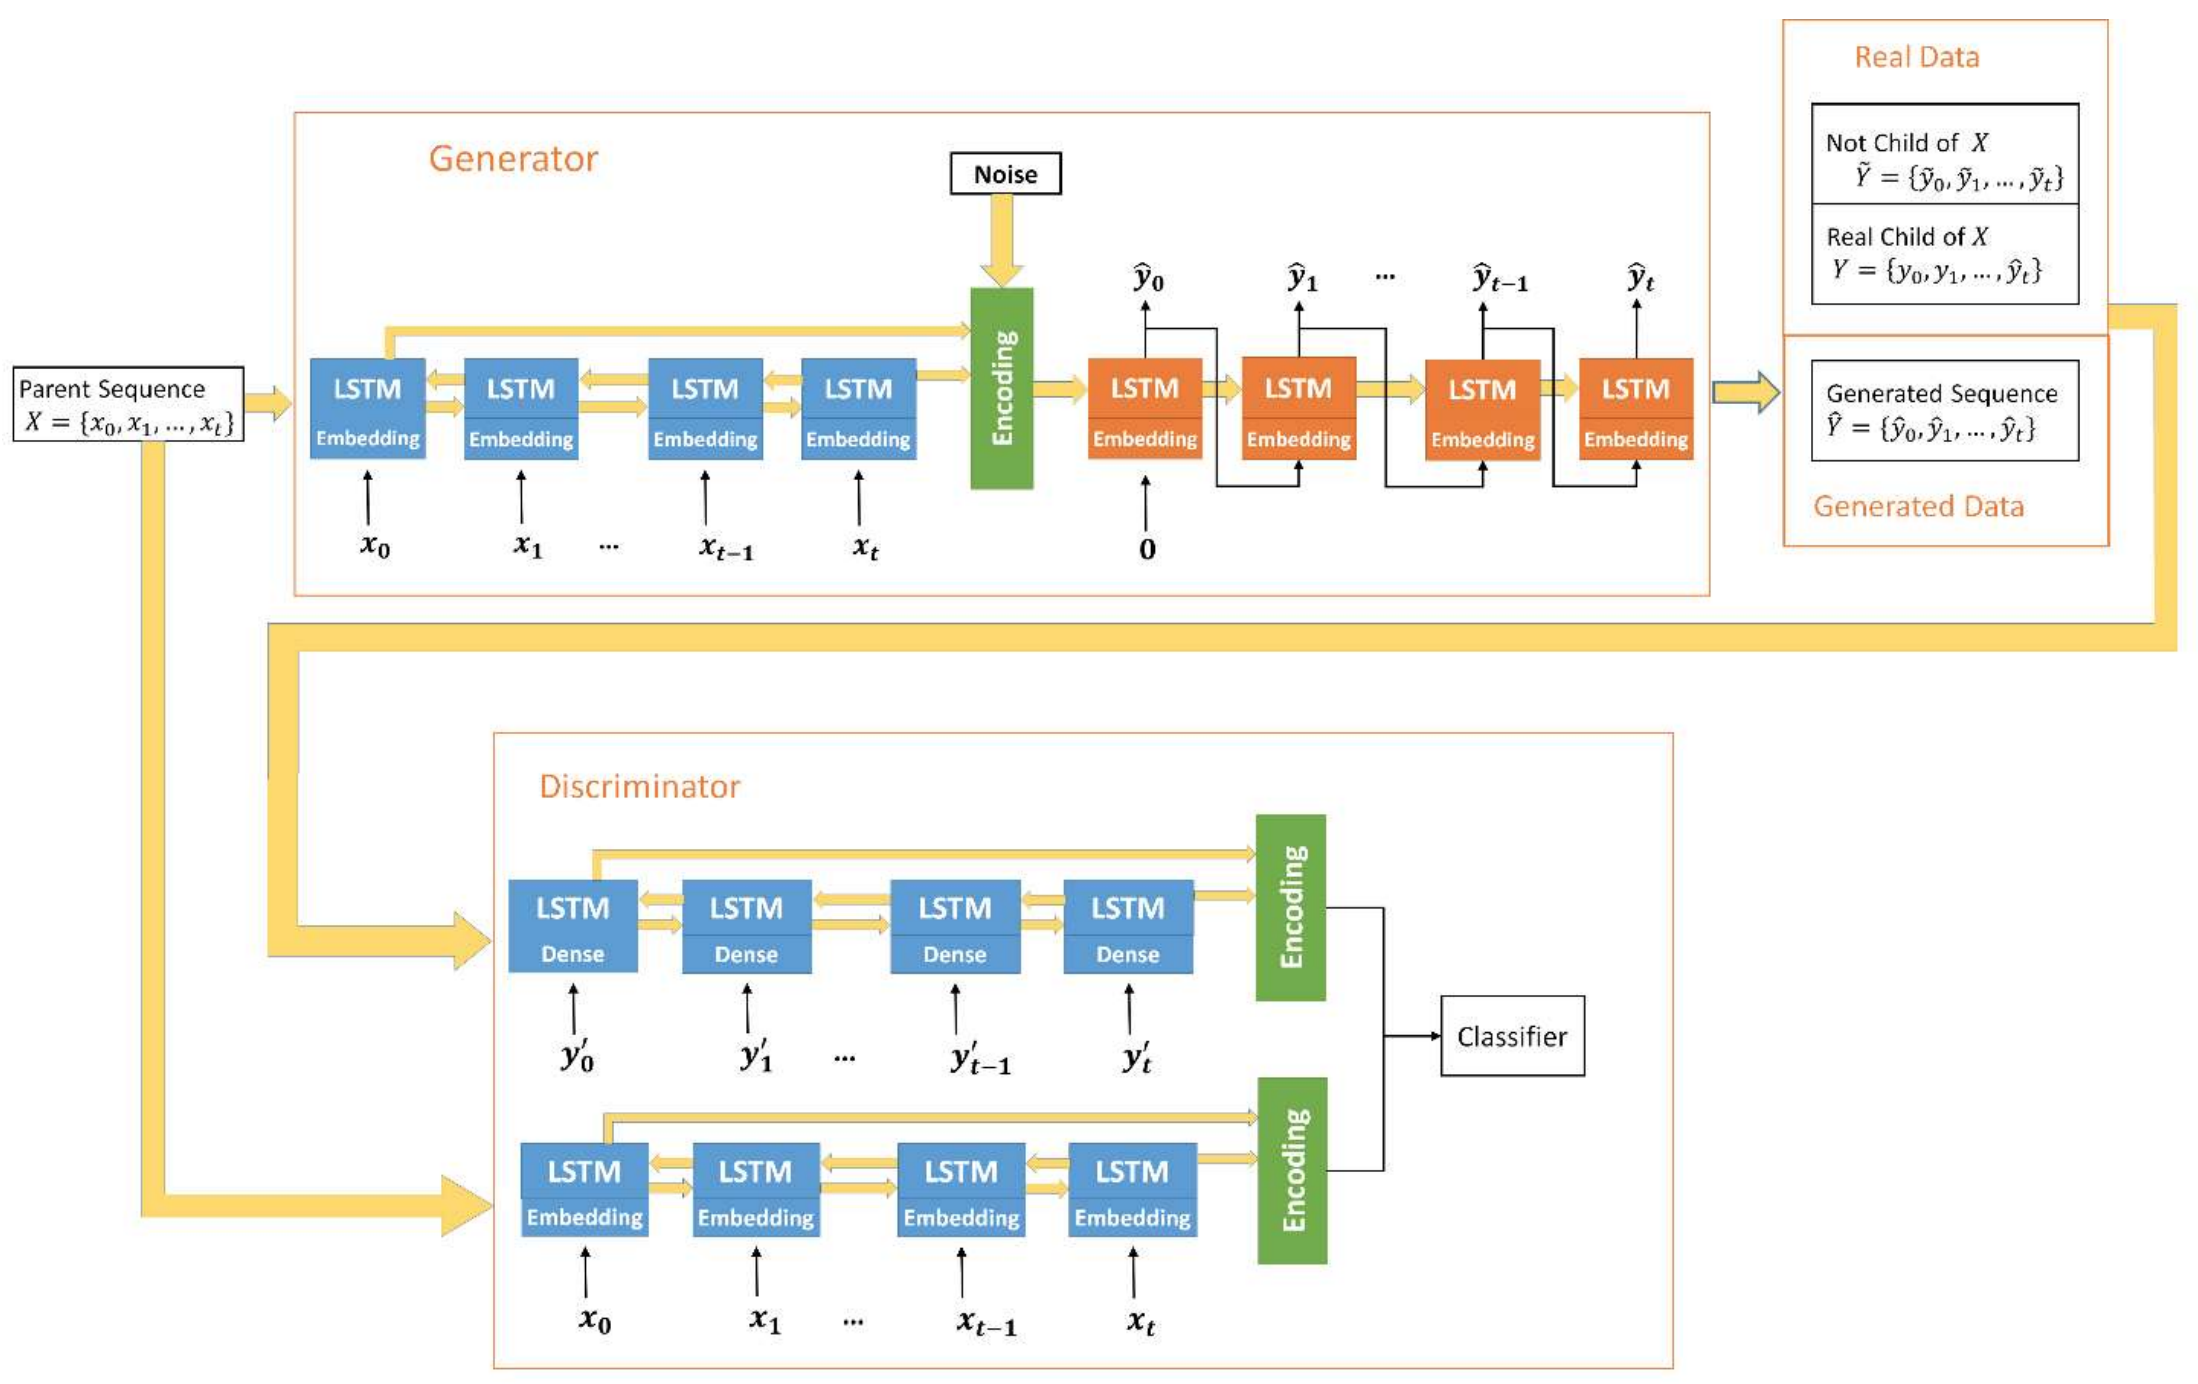
\includegraphics[width=\linewidth]{figures/mutagan.png}
	\caption{Architecture of MutaGAN \cite{Berman2020}}
	\label{mutagan}
\end{figure}

MutaGAN's generator consists of a sequence to sequence model. The encoder is built from of a bidirectinal \ac{LSTM} and the resulting context vector of dimensionality 512 is combined with noise from a standard normal distribution. The decoder \ac{LSTM} predicts the resulting sequence of amino acids greedily using the $argmax()$ of the $softmax()$ output for every time step. The discriminator is trained on three different parent-child pair configurations to optimally compete against the generator, real parent-child pairs, real parent and generated child pairs and pairs of real sequences that are not parent-child pairs. Two bidirectional \ac{LSTM} encoders sharing the same weight matrix as the encoder of the generator produce a fixed-dimensional encoding of the provided parent-child pair used for classification of evolutionary descent by a plain neural network. The child encoder in the discriminator uses a dense layer having the same weight matrix as the embedding layer of the encoder of the generator. The dense layer is required to directly input the predicted child sequence as its probability distribution rather than the final output after applying the $argmax()$ as it would not enable backpropagation to train the generator. In case of a true child sequence is given a simple one-hot encoding is used. \cite{Berman2020}

Interestingly \cite{Berman2020} states planned improvements by utilizing bigger datasets aquired from the \ac{GISAID} database EpiFlu and by using more length-robust attention-based models to directly work on nucleotide sequences instead of sequences of amino acids. Therefore transformers and the attention mechanism are introduced in the following section.

\subsection{Transformer and Attention Mechanism} \label{fundamentalsG}

Using a sequence to sequence model as introduced based on an encoder-decoder architecture of \ac{LSTM} cells has some drawbacks. First the input needs to be process sequentially in time steps which makes parallelization difficult and increases training time, especially for longer sequences. Furthermore the hidden and cell state vector passed through every timestep tries to encode information of all previous time steps without knowing which information is especially inportant for the current time step. This not only makes long distance dependencies hard to capture, but also might not get the prioritization of the previous time step inputs right. 

To tackle these problems the so-called transformer architecture was introduced in \cite{Vaswani2017}. It feeds an entire sequence into the encoder to be processed in parallel denying any concept of recurrence or convolution. Only using a so called self-attention mechanism the transformer makes sure that during processing every input position, each of them receives the information that is most important to them. This way modeling long dependencies becomes much more easy compared to \acp{LSTM} as the view on the input sequence is more global. In this architecture, the encoder also passes all computed hidden states of every position to the decoder, which therefore can generate the target sequences based on more semantically enriched features and also in parallel for every position. \cite{Vaswani2017}

The transformer architecture achieved state-of-the-art quality results with a BLEU score of 41.8 on the WMT 2014 English-to-French translation task (cf. BLEU score of \cite{Sutskever2014} was 34.8), while still being much faster to train due to its parallelization capabilities. State-of-the-art results are already achieved after just twelve hours of training on eight P100 \acp{GPU}. As this is still far beyond the scope and resources given for this project, this projects provides a proof-of-concept transformer model trained for far shorter and fewer sequences as one would need to predict entirely new \ac{RNA} sequences. \cite{Vaswani2017}

First the transformer architecture should be introduced in the following:

\begin{figure}[ht]
	\centering
	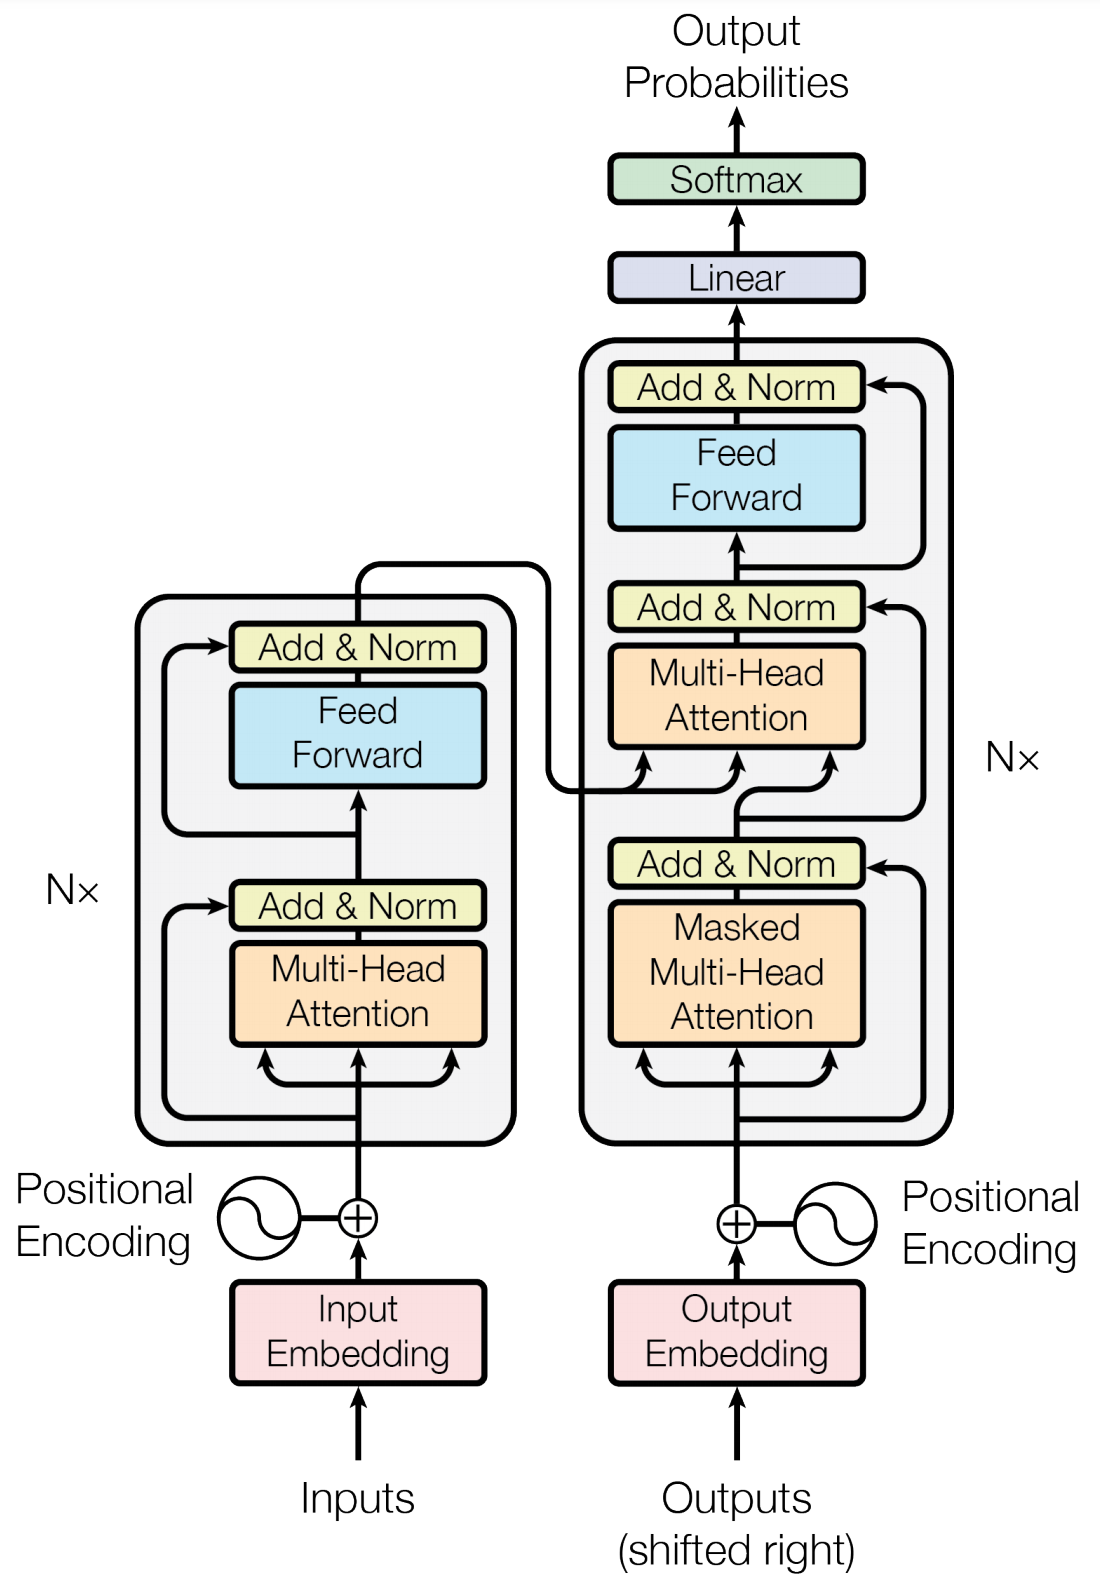
\includegraphics[width=0.5\linewidth]{figures/transformer.png}
	\caption{Architecture of the transformer \cite{Vaswani2017}}
	\label{transformer}
\end{figure}

The transformer consists of an encoder and a decoder part just as normal sequence to sequence models. One layer of the encoder contains a self-attention layer before passing the hidden state representations of an input sequence to a feed forward neural network. Thus it makes sure that semantic and contextual dependencies between different positions in the input sequence are also modeled. Also skip connections are added for both components with subsequent layer normalization. \cite{Alammar2018}

To calculate the self-attention ouput of a sequence, a query $Q$, key $K$ and value $V$ matrix is calculated through multiplication of the sequence representation\footnote{A matrix containing the hidden state representations of every input position} with learned transformation matrices. Each row of the three received matrices corresponds to a specific input position. The output of the self-attention layer is then calculated through

\begin{equation}
	(Scaled Dot-Product) Attention(Q, K, V) = softmax(\frac{QK^T}{\sqrt{d_k}})V.
\end{equation}

The dot product between $Q$ and $K$ calculates scores that are used as weighting factors for $V$. This models for every input position how relevant all other input positions are for each of the hidden state encodings. The scores are divided by the square root of the dimensionality of the query/key/value values of the hidden state representations, which is chosen to be 64 (square root eight), to receive more stable non-vanishing gradients. The softmax guarantees that the positional scores lie between zero and one and add up to one. Note that the score of the current input position itself will most likely have the hightest score. \cite{Alammar2018}

\begin{figure}[ht]
	\centering
	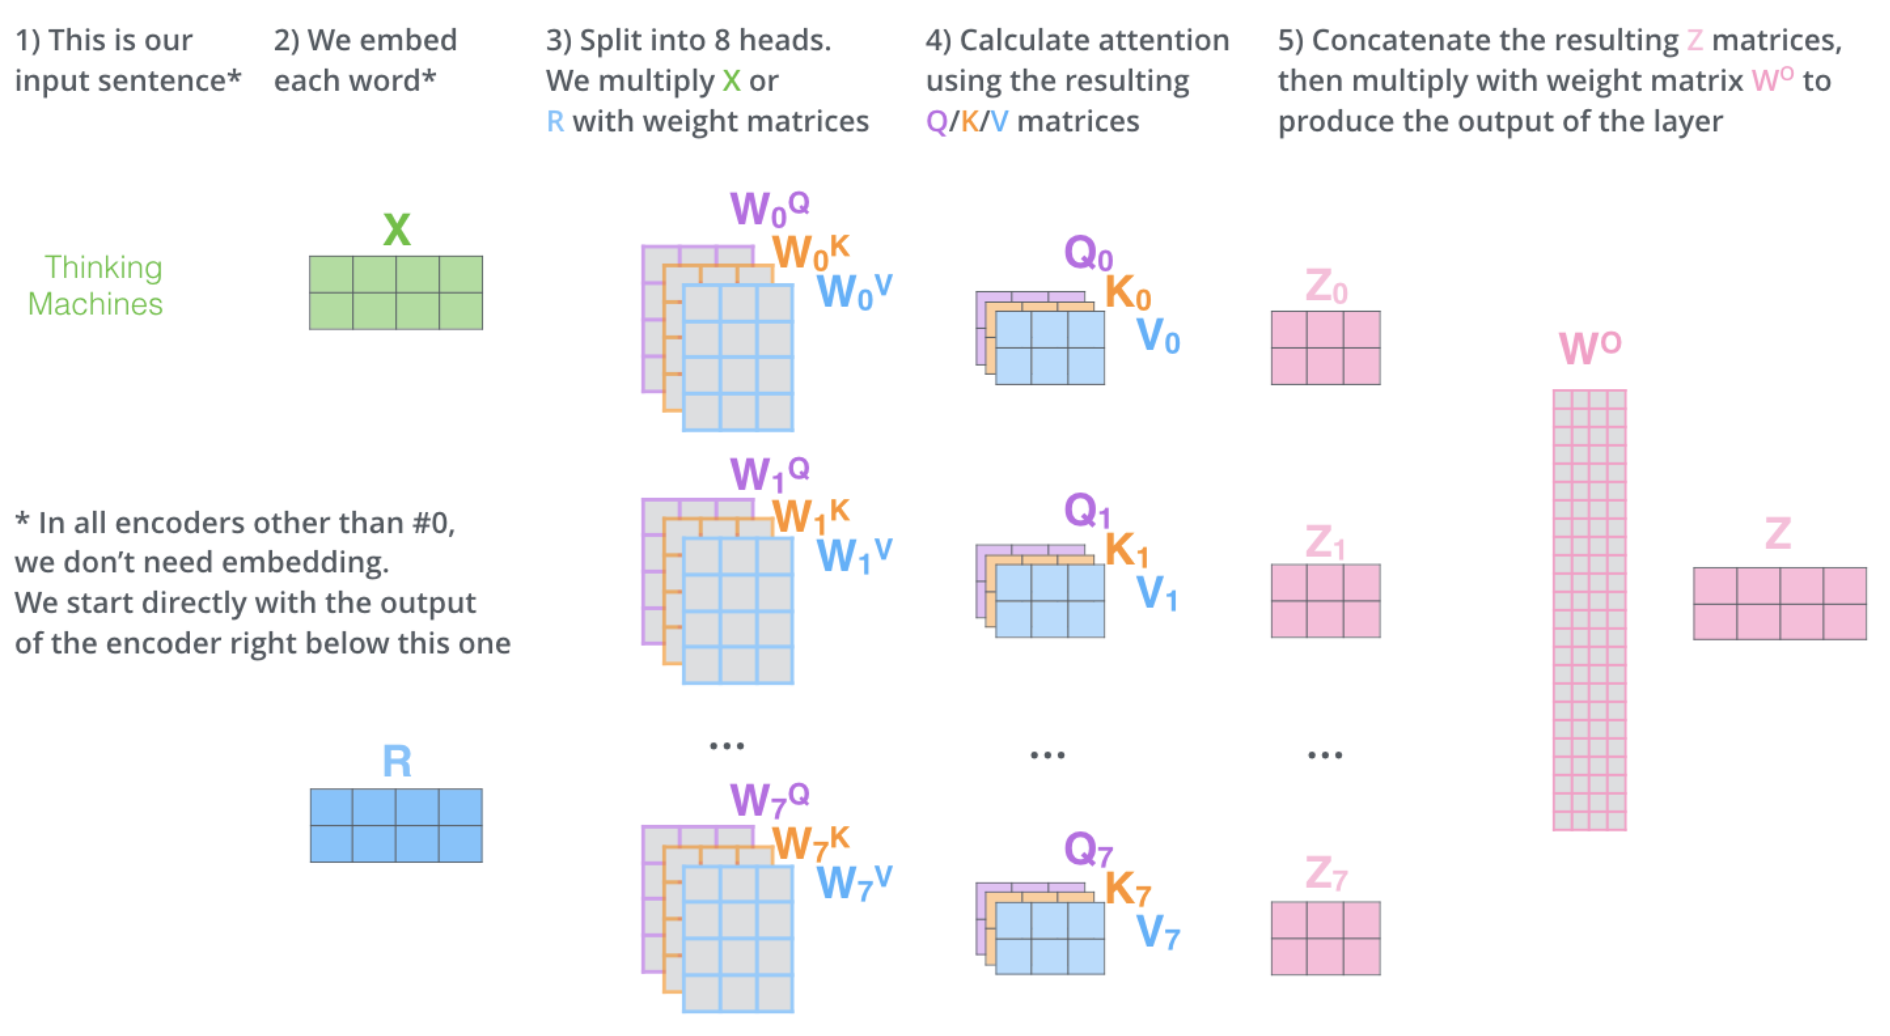
\includegraphics[width=\linewidth]{figures/multi_head_attention.png}
	\caption{Multi-head attention architecture \cite{Alammar2018}}
	\label{multi-head-attention}
\end{figure}

One can expand self-attention towards a multi-head attention. In this configuration each head produces its own query, key and value matrices and therefore its own self-attention output. The resultung hidden state is calculated by concatenating each hidden state output of the different heads and multiplying it with a contraction matrix that outputs a hidden state vector in its single-head dimensionality. Multi-head attention is needed to be able to better focus on multiple parts of the input sequence when encoding an input position, otherwise it might happen that most of the focus is set on the input position itself. \cite{Alammar2018}

Overall six layers of encoder and decoder components having individual weight matrices are stacked on top of each other to capture low-level as well as high-level features. The dimenionality of the hidden state is 512. Note that each position of the input sequence is encoded on an individual path throught the transformer, which makes parallelization possible compared to \ac{LSTM} based architectures. \cite{Alammar2018}

The decoder uses almost the same architecture as the encoder, but contains an additional multi-head attention component that integrates all the hidden state encodings from the encoder. Therefore the final hidden state encodings resulting from the top most encoder are transformed into key and value attention vectors and given to the integrating mutli-head attention component of every decoder. Once again this helps to better focus on the relevant input positions for the current output position based on hidden state information extracted from the encoder. Note that the decoder works in a sequential manner again meaning that the input to the decoder are the already decoded sequence tokens of previous time steps, future input positions are masked away. The first multi-head attention component therefore capture inter-dependencies in the generated output sequence, the second one enriches the hidden state encoding with the information given from the encoder hidden states. Finally a linear layer mapping the hidden state vector to a logits vector with dimensionality of the given output dictionary and a $softmax()$ function produce the output sequence using the greedy or beam search approach. The \textit{EOS} token symbolizes the end of the output to be generated. \cite{Alammar2018}

Input to the transformer are word embeddings also of fixed dimensionality of 512. Onto each word embedding a positional encoding following a specific pattern is added. These patterns are learned and make sure that the distances of the input positions are projected onto the queue, key and value representations to be utilized during scaled dot-product attention. This also enables self-attention to be scaled to unseen lengths of sequences. Transformers usually contain an upper bound of sequence length to be processed, which is different to recurrent architectures that can process inputs of arbitrary length. Input sequences are usually padded up until the specified sequence length, the used \textit{PAD} tokens are masked to be excluded from the self-attention components. \cite{Alammar2018}

% One is the total computational complexity per layer. Another is the amount of computation that can be parallelized, as measured by the minimum number of sequential operations required. The third is the path length between long-range dependencies in the network.

\subsection{Other Techniques} \label{fundamentalsH}

\begin{itemize}
	\item NNs/SVMs: \url{https://bsb-eurasipjournals.springeropen.com/articles/10.1186/s13637-016-0042-0}
	\item BiLSTM: \url{https://science.sciencemag.org/content/371/6526/284}
\end{itemize}


\newpage

%\section{Approach} 
\label{approach}

Figure \ref{pipeline} visualizes the steps of our approach, which are described in detail in the following chapters.

\begin{figure}[ht]
	\centering
	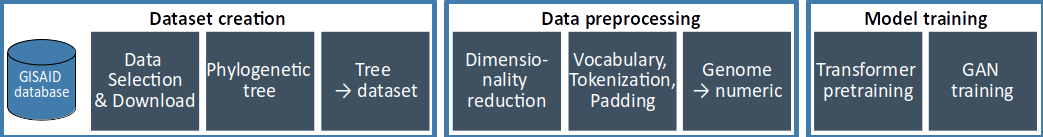
\includegraphics[width=1.0\linewidth]{figures/pipeline.png}
	\caption{Approach pipeline \cite{own representation}}
	\label{pipeline}
\end{figure}


\subsection{Dataset Creation}  \label{ch:approachA}
% Choosing latest mutations that are the most spread
% Created three types of sequence pairs: (real, real), (real, generated), (real, unreal)
% Phylogenetic tree with "Fasttree"
% Levenshtein distance
% Biopython packages?
% Final dataset metrics

As described in chapter \ref{fundamentalsC} a dataset consisting of parent-child pairs is needed to learn a \ac{ML} model for mutation prediction. The steps to create this dataset are described in the following chapters.

\subsubsection{Raw data selection from \ac{GISAID}}
\label{ch:approachAa}

In the first step of the dataset creation the raw genomes and their metadata are downloaded from \ac{GISAID}. Therefore a selection of a suitable subpart of the data is necessary. The \ac{GISAID} platform only allows the download of 5000 genomes at once. That is why we decided to focus our analysis on Germany (for one country the selection of < 5000 genomes is rather simple compared to the selection of data from multiple countries). By looking at the latest "Report on virus variants of SARS-CoV-2 in Germany" from the \ac{RKI} we decided for a time period. Figure \ref{rkiVariantDistribution} shows the distribution of different variants over time. Starting from calendar week 18 the Delta variant gradually displaces the previously widespread Alpha variant.

\begin{figure}[ht]
	\centering
	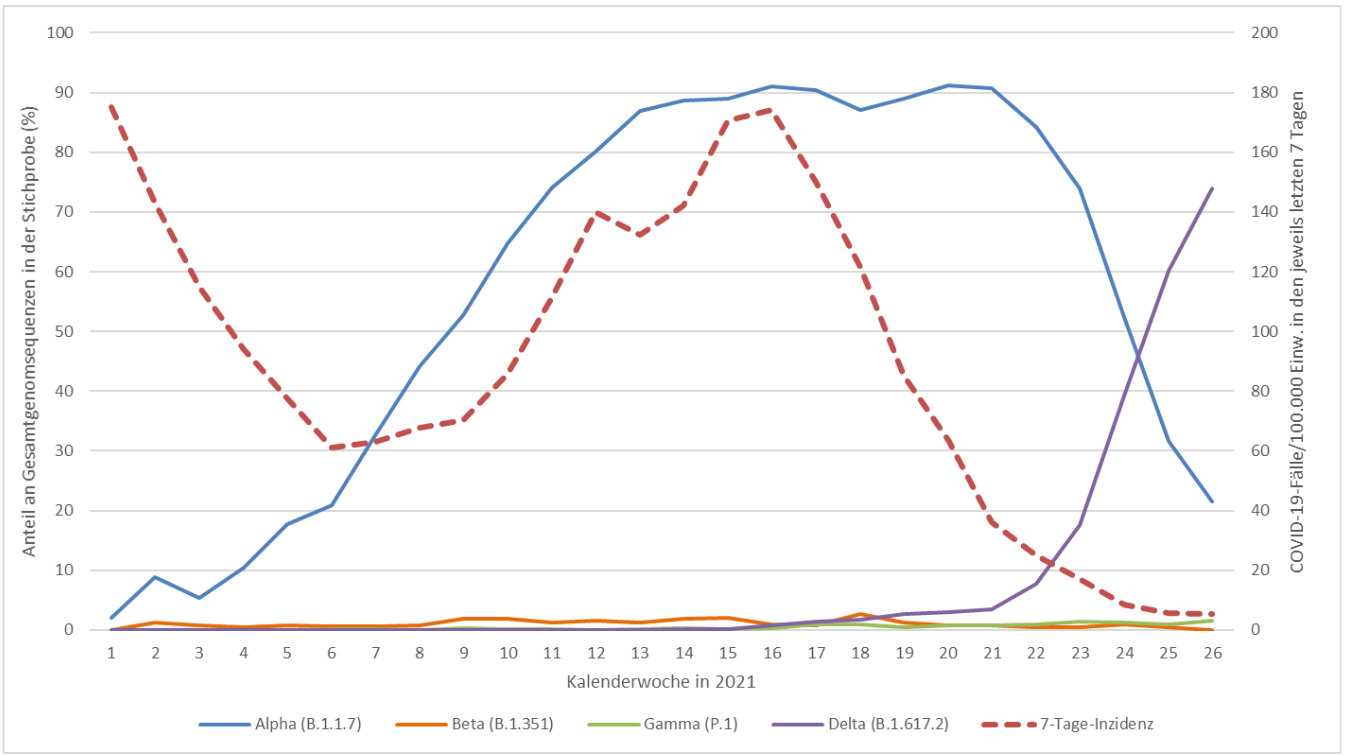
\includegraphics[width=1.0\linewidth]{figures/rkiVariantDistribution.png}
	\caption{Variant distribution in Germany over time \cite{robertkochinstituteditorBerichtVirusvariantenSARSCoV22021}}
	\label{rkiVariantDistribution}
\end{figure}

That is why we selected the data from 04.05.2021 (calendar week 18) until 15.07.2021 (calendar week 28). This results in a raw dataset of 35.818 genomes.
Each genome consists of a FASTA file containing the genomes sequence and a record in a tsv file with the metadata.

%TODO: beispiel record: genome sequence and metadata


\subsubsection{Generation of a phylogenetic tree}
\label{ch:approachAb}

As described above we need parent-child genome sequence pairs to be able to train a \ac{ML} model. Therefore we need to evaluate the ancestral relationships between the genome sequences.
As described in chapter \ref{fundamentalsA0d} this is done in biology through phylogenetic trees.
For the data preparation (e.g. alignment) and the calculation of the phylogenetic tree we use the nextstrain pipeline \cite{10.1093/bioinformatics/bty407}.
The pipeline was executed on a local computer with Intel Core i7-7500U (4*2.70GHz), NVIDIA GeForce 940MX and 16 GB RAM.
Unfortunately after two days of calculation, the nextstrain pipeline exited with an out of memory exception. That is why the amount of data is decreased. This was done through iterative reduction of the dataset size. The largest locally computable dataset consists of 11.773 genome sequences.

The generated phylogenetic tree can be seen in figure \ref{phylogeneticTree}.
%TODO: Beschreibung was man sieht

%TODO: nicer tree image?
\begin{figure}[ht]
	\centering
	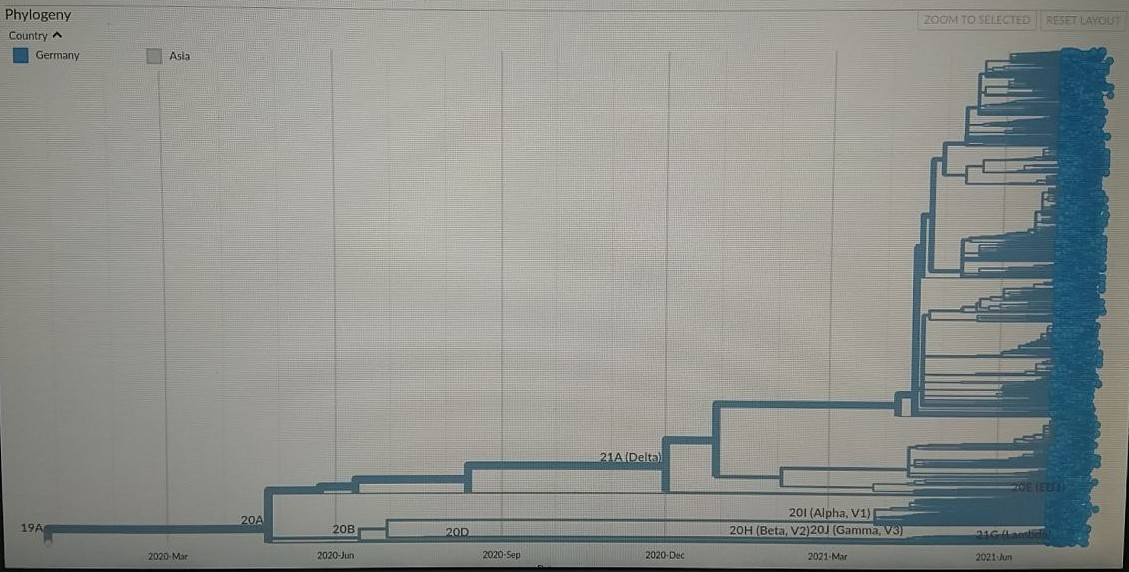
\includegraphics[width=1.0\linewidth]{figures/phylogeneticTree.jpg}
	\caption{Phylogenetic tree of our dataset \cite{own representation}}
	\label{phylogeneticTree}
\end{figure}

\subsubsection{Phylogenetic tree to dataset}
\label{ch:approachAc}

Based on the calculated phylogenetic tree the final dataset is generated. Therefore the patristic distances between all leaf nodes are calculated. From the resulting patristic distance matrix for each leaf node the most related next leaf node can be evaluated. The two leaf nodes with the smallest distance are the closest relatives to each other and therefore represent a parent-child pair. After the evaluation which leaf nodes are one parent-child pair, the question which node is the parent and which node is the child is clarified. Therefore the two nodes are sorted by their date, which is stored in the metadata file. The older genome sequence is the parent and the younger genome sequence is the child.

For calculating the patristic distance matrix we first used Dendropy (version: 4.5.2) \cite{DendroPyPhylogeneticComputing}. Again this leads to problems due to limited RAM on our local computer. As a consequence we switched to PhyloDM (version: 1.3.1) \cite{aaron_mussig_2020_4089111}, which is a library for calculating patristic distances in a memory and time efficient manner.

Finally we received a dataset containing parent-child genome sequences.

\subsection{Data Preprocessing}  \label{ch:approachB}
% TODO: Pipeline image
% Word size 3 is just a hyperparameter (see discussion of the corresponding paper)!  But maybe biologically valid because auf amino acids.
% DNA2Vec?

\subsubsection{Dimensionality reduction by selecting subpart of the genome}
\label{ch:approachBa}

The full \ac{SARS-CoV-2} genome consists of about 30.000 nucleotides. Due to the limited computing capacity on our local computers we need to reduce the dimensionality of the dataset. This is done by selecting a subpart based on the gained data insights from chapter \ref{ch:experimentsA}. In figure \ref{mutatedGeneticLoci} parts of the genome with lots of mutations are visible. Based upon this we selected 99 nucleotides (33 codons) in the range between position 21.800 and 21.899.

\subsubsection{Transform genome sequence to numeric model input}
\label{ch:approachBb}

Input to the model are numericalized codon sequences with each codon being composed of three nucleotides. Therefore one needs to build a vocabulary with all codons existing in the dataset that assigns each codon a unique number. Each genome string is therefore tokenized to codons and so far unseen codons are added to the vocabulary. The vocabulary also contains special tokens like:

\begin{itemize}
	\item \textit{<SOS>}: start of sentence
	\item \textit{<EOS>}: end of sentence
	\item \textit{<UNK>}: unknown
	\item \textit{<PAD>}: padding
\end{itemize}

A codon is encoded as unknown in case at least one nulceotide is unknown or at least one padding character is contained. Only in the special case of three padding characters the padding token is returned. 

To integrate the dataset into the training routine, PyTorchs \textit{DataLoader} is used (see \autoref{ch:approachD}). Therefore a \textit{CustomGISAIDDataset} class is derived from PyTorchs Dataset class that can be utilized by the \textit{DataLoader}. It can be configured to return the training or test dataset instances. Each instance is already numericalized by vocabulary index lookups for each codon, padded with the numericalized \textit{<SOS>} and \textit{<EOS>} token and transformed to a PyTorch tensor. 

\subsection{Model Architecture}  \label{ch:approachC}

The connection of modeling evolution theory of virus mutations to probabilistic language modeling has already been explained in \autoref{fundamentalsA}. To create such a probabilistic language model an approach closely related to the one introduced by the MutaGAN paper \cite{Berman2020} as explained in \autoref{fundamentalsF} is chosen with the novelty that attention-based transformers are used instead of \acp{LSTM}\footnote{This improvement was also named in the conclusion of the MutaGAN paper.}. To implement the \ac{GAN} framework PyTorch is used as it provides full-featured classes for transformers, embedding layers and other architectural components needed. This way one can specialize on the training routine instead of implementing a custom transformer architecture, which might be too error-prone\footnote{In case one is interested in how to implement a custom transformer architecture, see \url{http://nlp.seas.harvard.edu/2018/04/03/attention.html}.}. 
% Give further explanations here

The numericalized codon sequences first need to be transformed to input embeddings. Therefore ...

% Hyperparameters and model architecture
% Reverse sequences?

\subsection{Training Process} \label{ch:approachD}

TODO

% Plot accuracy and loss for training and validation
% Loss functions and teacher forcing, early stopping?
% Categorical cross-entropy loss for seq2seq, Wasserstein loss for GAN, kullback leibner + cross entropy for transformers
% Identify changes between sequences using the diff-match package from Google
% See MutaGAN 6.2 Model training
% Replay buffer
% Dealing with the mode collapse problem

\newpage

%\section{Experimental results} \label{experiments}

\subsection{Dataset insights}  \label{ch:experimentsA}

This chapter presents the dataset insights of the complete dataset with full genome sequences and the dataset insights of the preprocessed dataset.

\subsubsection{Complete dataset}  \label{ch:experimentsAa}

\begin{wrapfigure}{R}{8cm}
	\centering
	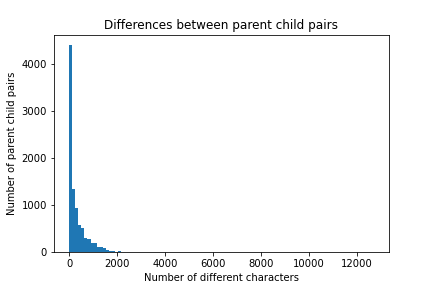
\includegraphics[width=0.9\linewidth]{figures/distributionDifferencesParentChild.png}
	\caption{Distribution of the differences between parent and child sequences \cite{own representation}}
	\label{distributionDifferencesParentChild}
\end{wrapfigure}

The dataset consists of 9199 parent-child pairs.
The distribution how the parent and child sequences differ can be seen in figure \ref{distributionDifferencesParentChild}. The majority of parent-child pairs differ in less than 200 characters. The number of completely equal parent-child pairs is 396.

\vspace{2cm}
Figure \ref{mutatedGeneticLoci} visualizes the distribution of mutations over the full \ac{SARS-CoV-2} genome.

\begin{figure}[ht!]
	\centering
	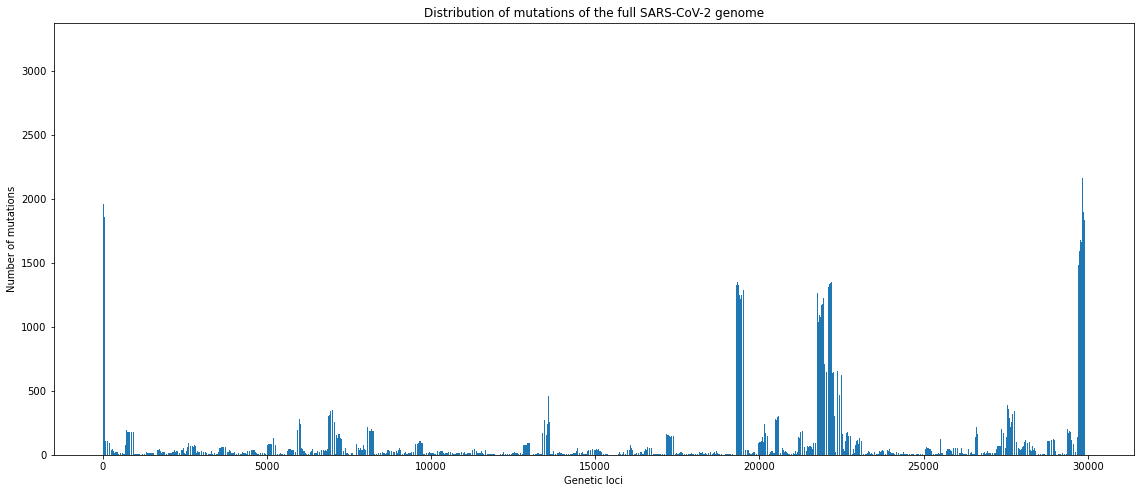
\includegraphics[width=1.0\linewidth]{figures/mutatedGeneticLoci.png}
	\caption{Mutated genetic loci \cite{own representation}}
	\label{mutatedGeneticLoci}
\end{figure}

\newpage
\subsubsection{Preprocessed dataset}  \label{ch:experimentsAb}

The complete dataset is preprocessed as described in chapter \ref{ch:approachB}. The distribution how the parent and child amino acids differ in the selected subpart can be seen in figure \ref{preprocessedDistributionDifferencesParentChild}. The majority (6946) of parent-child pairs are equal. This is not optimal for training the \ac{ML} model and is further discussed in chapter \ref{ch:experimentsB}. 

\begin{figure}[ht]
	\centering
	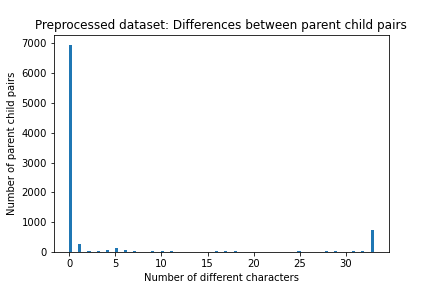
\includegraphics[width=0.6\linewidth]{figures/preprocessedDistributionDifferencesParentChild.png}
	\caption{Preprocessed dataset: Distribution of the differences between parent and child sequences \cite{own representation}}
	\label{preprocessedDistributionDifferencesParentChild}
\end{figure}

Figure \ref{preprocessedMutatedGeneticLoci} visualizes the differing amino acids and their positions of the selected subpart of the \ac{SARS-CoV-2} genome. They are distributed equally over the selected subpart.

\begin{figure}[ht]
	\centering
	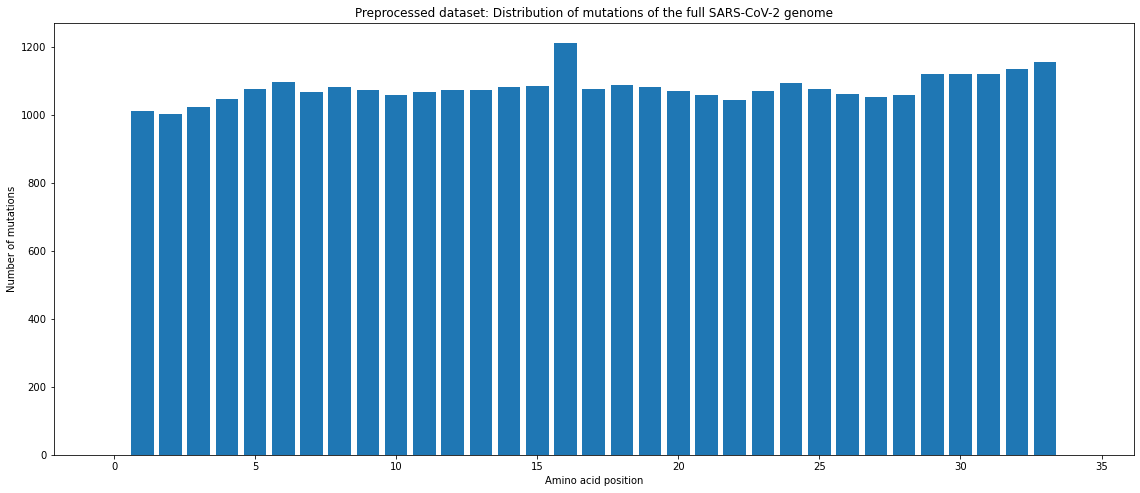
\includegraphics[width=0.9\linewidth]{figures/preprocessedMutatedGeneticLoci.png}
	\caption{Preprocessed dataset: Differing amino acid positions \cite{own representation}}
	\label{preprocessedMutatedGeneticLoci}
\end{figure}

\newpage
\subsection{Evaluation}  \label{ch:experimentsB}

\subsubsection{Evaluation criteria}

To measure the success of the transformer model different evaluation criteria need to be introduced that capture how well the mutations observed in the data can be reproduced by the generator. A mutation prediction is considered correct in case the prediction matches in codons and locations. Further to distinguish are partially correct mutation predictions in case mutations are observed at the right locations but in different codons. Mutation predictions can further be considered as wrong in case they were not observed in the true child sequences or missed in case they could not be observed in the generated sequences. 

A common metric used in the domain of \ac{NMT} is the so-called \ac{BLEU} score \cite{Papineni2002}. Its so-called modified n-gram precision captures common n-grams between the generated sentence and the true reference translation sentence independently of their position. Also a sentence brevity penalty is incorporated into the score. The \ac{BLEU} score ranges between zero and one with one being a perfect match to the reference translation. \cite{Papineni2002}

Using solely the \ac{BLEU} score would mean less focus on the concrete mutation prediction at critical genome positions but rather a correct overall child sequence prediction. As the child sequence is mostly similar to the parent sequence, predicting a nearly identical child sequence is not too difficult and the \ac{BLEU} score would resolves already to a high value at early stages of training. 

Therefore the MutaGAN paper \cite{Berman2020} introduced several other metrics besides the \ac{BLEU} score. For instance the distribution of specific codon mutations between the ground truth data and the generated data was calculated to evaluate the similarity of both mutation profiles. Furthermore a so-called sequence true positive rate is determined by capturing all observable predicted mutations for each parent sequence and comparing them to the list of actual existing mutations for each parent sequence in the ground truth data. 

Besides the \ac{BLEU} score, we also utilize the sequence true positive rate to evaluate the model using Google's \textit{Diff Match and Patch} libraries to identify the mutations\footnote{For the Diff Match and Patch libraries, see \url{https://github.com/google/diff-match-patch}}. The Levenshtein distance to determine the degree of similarity between a parent and generated child sequence is not used as at most two mutations appear for a given parent genome during the evaluation phase making the Levenshtein distance neglectible. 

\subsubsection{Training phase and evaluation}  \label{ch:experimentsBa}

Figure \ref{pretrainingLossPlot} shows the loss plot for the transformer pretraining. The model converges rather fast. Similar is the actual \ac{GAN} training (see \ref{trainingLossPlot}). 

\begin{figure}[ht]
	\centering
	\begin{subfigure}[b]{0.49\textwidth}
		\centering
		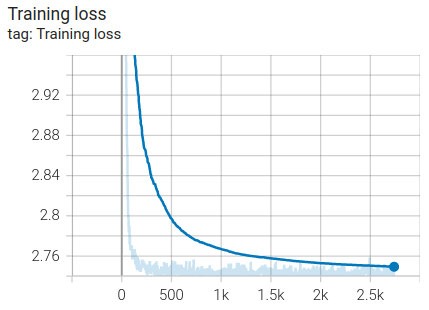
\includegraphics[width=\linewidth]{figures/pretrainingLossPlot.png}
		\caption{Transformer pretraining loss plot}
		\label{pretrainingLossPlot}
	\end{subfigure}
	\hfill
	\begin{subfigure}[b]{0.49\textwidth}
		\centering
		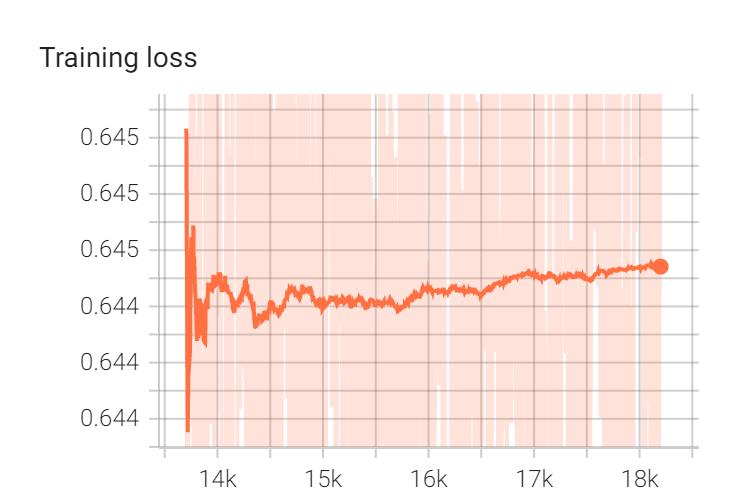
\includegraphics[width=\linewidth]{figures/trainingLossPlot.png}
		\caption{Transformer training loss plot}
		\label{trainingLossPlot}
	\end{subfigure}
\end{figure}

Whereas the trained model achieves a relatively high \ac{BLEU} score with 87.42\%, the sequence true positive rate only amounts to 31\%. Thus one concludes that the model generates reasonable and close genomes from given parent sequences, but at first glance develops only partly the capability to predict the actual and correct mutations given in the ground truth data. When further analyzing the rather low sequence true positive rate, one recognizes that a lot of false predictions where made that can be traced back to cases where the parent sequence consists of a series of \textit{<UNK>} tokens that are replaced by actual codons. As these kinds of mutations are not present in the ground truth data, whose matching child pairs still contain the \textit{<UNK>} series, one can think of an additional capability of the trained transformer model as a gap filler of unknown sequence parts of parent genomes, that is even beneficial. Other mutations where captured really well, e.g. from codon \textit{TTG} to \textit{CTG} at strang location 45 or from codon \textit{G} to \textit{A} at strang location x. During evaluation at most two mutations on the same parent in one prediction appeared, matching to the actual ground truth. Some mutations in the ground truth data were also missed, especially in case they were not too frequent. During evaluation only 25 unique parent sequences were considered in the test dataset further reducing a diverse prediction capability of the model. But as data selection and preprocessing is very time and especially resource extensive\footnote{Phylogenetic tree reconstruction might take several days until completion.}, the scope of the project and its data used is intenionally kept minimal to provide a proof of concept. In this sense, on can conclude that the model first not only generates reasonable genome strang offsprings, but also embodies noticable codon mutations of the ground truth data. When up-scaling the amount of genome sequences to use and doing more strict filtering of genome sequences to increase the data quality, predicting virus mutations using transformers is very well feasible. As a comparison MutaGAN achieves a \ac{BLEU} score of 97.46\% and an unweighted sequence true positive rate of just 21\% \cite{Berman2020}. 
 
\newpage


\clearpage
\pagenumbering{Roman}
% \appendix
% \section{Appendix}

\subsection{Appendix A}
\label{ch:app-A}


%%%%%%%%%%%%%%%%%%%%%%%%%%%%%%%%%%%%%%%%%%%%%%%%%%%%%%%%%%%%

\newpage
\printbibliography

\end{document}
